\documentclass[a4paper,12pt]{article}

%%% Работа с русским языком
\usepackage{cmap}					% поиск в PDF
\usepackage{mathtext} 				% русские буквы в формулах
\usepackage[T2A]{fontenc}			% кодировка
\usepackage[utf8]{inputenc}			% кодировка исходного текста
\usepackage[english,russian]{babel}	% локализация и переносы

%%% Страница
\usepackage{extsizes}               % Возможность сделать 14-й шрифт
\usepackage{geometry}               % Создание полей
\geometry{top = 2cm}
\geometry{bottom = 2cm}
\geometry{left = 2.5cm}
\geometry{right = 2.5cm}

\renewcommand{\baselinestretch}{1.5} % Интерлиньяж 1.5

\usepackage{hyperref}                % Ссылки
\usepackage{cite}                    % Цитаты
\usepackage{indentfirst}             % Абзацы
\usepackage[nottoc,numbib]{tocbibind}

%%% Дополнительная работа с математикой
\usepackage{amsmath,amsfonts,amssymb,amsthm,mathtools} % AMS
\usepackage{icomma} % "Умная" запятая: $0,2$ --- число, $0, 2$ --- перечисление

%% Номера формул
%\mathtoolsset{showonlyrefs=true} % Показывать номера только у тех формул, на которые есть \eqref{} в тексте.
%\usepackage{leqno} % Нумерация формул слева

%% Свои команды
\DeclareMathOperator{\sgn}{\mathop{sgn}}

%% Перенос знаков в формулах (по Львовскому)
\newcommand*{\hm}[1]{#1\nobreak\discretionary{}
	{\hbox{$\mathsurround=0pt #1$}}{}}

%%% Работа с картинками
\usepackage{graphicx}            % Для вставки рисунков
\graphicspath{{pictures/}}       % папки с картинками
\setlength\fboxsep{3pt}          % Отступ рамки \fbox{} от рисунка
\setlength\fboxrule{1pt}         % Толщина линий рамки \fbox{}
\usepackage{wrapfig}             % Обтекание рисунков текстом
\DeclareGraphicsExtensions{.pdf,.png,.jpg}
\usepackage{float}

%%% Работа с таблицами
\usepackage{array,tabularx,tabulary,booktabs} % Дополнительная работа с таблицами
\usepackage{longtable}                        % Длинные таблицы
\usepackage{multirow}                         % Слияние строк в таблице

%%% Теоремы
\theoremstyle{plain}                          % Стиль по умолчанию
\newtheorem{theorem}{Теорема}[section]
\newtheorem{proposition}[theorem]{Утверждение}

\theoremstyle{definition}                     % "Определение"
\newtheorem{corollary}{Следствие}[theorem]
\newtheorem{problem}{Задача}[section]

\theoremstyle{remark}                         % "Примечание"
\newtheorem*{nonum}{Решение}

%%% Программирование
\usepackage{etoolbox}                         % логические операторы
\usepackage{lastpage}                         % Узнать, сколько всего страниц в документе.
\usepackage{soul}                             % Модификаторы начертания

%%% Библиография
\makeatletter
\bibliographystyle{bibliography/gost}         % Генерация по ГОСТу
\renewcommand{\@biblabel}[1]{#1.}             % Замена скобок на точку
\makeatother

\begin{document}
\renewcommand{\contentsname}{\Large Содержание}
\renewcommand{\bibname}{\normalfont\Large\bfseries Список литературы}

\begin{titlepage}
    \begin{center}
        Министерство науки и высшего образования Российской Федерации \\
        НАЦИОНАЛЬНЫЙ ИССЛЕДОВАТЕЛЬСКИЙ ЯДЕРНЫЙ УНИВЕРСИТЕТ <<МИФИ>> \\*
        \hrulefill
    \end{center}

    \begin{center}
        ИНСТИТУТ ЛАЗЕРНЫХ И ПЛАЗМЕННЫХ ТЕХНОЛОГИЙ\\
        КАФЕДРА №31 ПРИКЛАДНАЯ МАТЕМАТИКА
    \end{center}
    \vspace{1cm}

    \vspace{2em}

    \begin{center}
        \large{Отчет}

        по проектной практике на тему:
    \end{center}

    \begin{center}
        \large СОЗДАНИЕ CNC СТАНКА
    \end{center}

    \vspace{20em}

    \begin{flushright}
        Работу выполнили: \\ Романов Сергей, Есис Александр, Никитин Кирилл\\
        Руководитель проекта: Морозов Андрей Андреевич
    \end{flushright}

    \vspace{5em}

    \begin{center}
        г. Москва 2022
    \end{center}
\end{titlepage}

\newpage
\tableofcontents
\setcounter{page}{3}

\newpage
\section*{Аннотация}

Данный этап работы по представленной теме является продолжением работы предыдущего семестра.
Все исходные коды и подпрограммы находятся на \href{https://github.com/AlexEsn/Project_CNC}{github}.

\section{Введение}

Современное состояние техники и производства характеризуется высоким уровнем автоматизации, применением сложнейших электронных устройств на основе компьютерных систем и комплексов.
Станки с ЧПУ - это компьютеризированные станки с числовым программным управлением, которые могут выполнять определенный набор операций в соответствии с заложенной в них программой.
Подобные станки могут управляться с помощью компьютеров (наиболее сложные станки) или микроконтроллеров
\cite{CNC_Plotter}.
Первым очевидным плюсом от использования станков с ЧПУ является более высокий уровень автоматизации производства. Случаи вмешательства оператора станка в процесс изготовления детали сведены к минимуму. Станки с ЧПУ могут работать практически автономно, день за днем, неделю за неделей, выпуская продукцию с неизменно высоким качеством. При этом главной заботой оператора являются в основном подготовительно-заключительные операции: установка и снятие детали, наладка инструмента и т.д.
Вторым преимуществом является производственная гибкость. Это значит, что для разных деталей нужно всего лишь заменить программу. А уже проверенная и отработанная программа может быть использована в любой момент и любое число раз.
Третьим плюсом является высокая точность. По одной и той же программе вы сможете изготовить с требуемым качеством тысячи практически идентичных деталей.
Таким образом, ЧПУ станок позволяет быстро получить спроектированное на компьютере изделие, причем ЧПУ станок производит изделия гораздо быстрее и качественнее чем вручную. Точный и легко приспосабливаемый ЧПУ станок позволяет осуществить проекты, которые, используя ручные технологии, оказались бы невыполнимыми или невыгодными \cite{sosonkin}.
К станкам ЧПУ относятся и плоттеры, которые могут рисовать какие-либо объекты по заданной программе.
Они представляет собой 2D-чертежные машины с 3D-управлением, которые используют перо для написания текста или рисования изображения на любом заданном твердом теле. ЧПУ плоттер можно использовать для таких целей, как проектирование печатных плат,
разработка логотипа, пирографии и др \cite{girhe_arduino_2018}.

\section{Цель и задачи}

Цель проекта: получить рабочий прототип портального ЧПУ станка.
Для достижения данной цели были поставлены следующие задачи:

\begin{enumerate}

    \item Изучение литературы и существующих моделей ЧПУ станков.
    \item Выбор наиболее подходящей модели.
    \item Создание 3D модели станка.
    \item Разработка и сборка электронной составляющей ЧПУ станка.
    \item Сборка и наладка первой простой рабочей модели.
    \item Усовершенствование полученной модели.

\end{enumerate}


\newpage
\section{Разработка модели}

При создании конструкции прорабатывались различные варианты, для этого использовалась матрица выбора.

\begin{table}[!ht]
    \centering
    \caption{Матрица выбора характеристик модели}
    \begin{tabular}{|p{3cm}|p{5cm}|p{2cm}|p{2cm}|p{2cm}|p{1cm}|}
        \hline
        Группы                 & Характеристика      & Простота в изготовлении & Удобство в эксплуатации & Удобная модернизация & Итог \\ \hline
        Стол                   & Подвижный стол      & 2                       & 4                       & 2                    & 8    \\ \hline
                               & Без стола           & 4                       & 2                       & 4                    & 10   \\ \hline
                               & Закрепленный стол   & 3                       & 5                       & 3                    & 11   \\ \hline
        Передача               & Передача винт-гайка & 5                       & 3                       & 2                    & 10   \\ \hline
        ~                      & Ременная передача   & 3                       & 4                       & 2                    & 9    \\ \hline
        ~                      & Зубчатая рейка      & 2                       & 4                       & 2                    & 8    \\ \hline
        Управляющий контроллер & Arduino             & 5                       & 5                       & 3                    & 13   \\ \hline
        ~                      & Raspberry           & 2                       & 5                       & 4                    & 11   \\ \hline
        Размер рабочего поля   & А4-А5               & 5                       & 3                       & 2                    & 10   \\ \hline
        ~                      & А4-А3               & 4                       & 5                       & 2                    & 11   \\ \hline
    \end{tabular}
\end{table}

После анализа вариантов с помощью матрицы выбора было принято решение по созданию портального ЧПУ станка со следующими характеристиками:
\begin{enumerate}
    \item Закрепленным столом, с передачей типа винт-гайка.
    \item Управляющий контроллер — Arduino Mega.
    \item Питание установки — 220В / 50 Гц. Питание прибора 12 VDC, 5 A.
    \item Размеры поля: 500×500 мм .
\end{enumerate}

Также предполагается разработка нескольких типов держателей для различных инструментов

\begin{figure}[H]
    \center{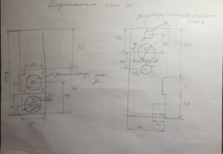
\includegraphics[scale=0.8]{2.png}}
\end{figure}

\begin{figure}[H]
    \center{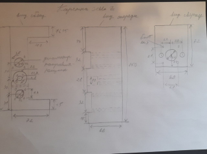
\includegraphics[scale=0.8]{3.png}}
    \caption{Первые чертежи}
\end{figure}


\begin{figure}[H]
    \center{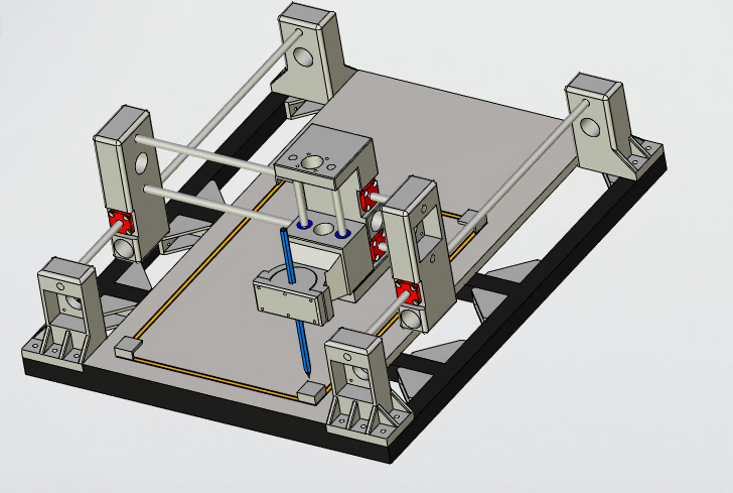
\includegraphics[scale=0.8]{1.png}}
    \caption{Стартовая модель станка}
\end{figure}

\newpage

Была составлена смета для определения недостающих деталей и их последующей закупки.

\begin{table}[!ht]
    \centering
    \caption{Смета для модели ЧПУ}
    \begin{tabular}{|p{7cm}|p{2cm}|p{2cm}|p{5cm}|}
        \hline
        Наименование                                             & Требуемое кол-во, шт & Стоимость, руб/шт & Ссылка                \\ \hline
        Электродвигатель шаговый 17HS4401S                       & 4                    & ---               & ---                   \\ \hline
        Arduino Mega                                             & 1                    & ---               & ---                   \\ \hline
        CNC Shield                                               & 1                    & ---               & ---                   \\ \hline
        Драйвер шагового двигателя А4988                         & 3                    & ---               & ---                   \\ \hline
        AC-DC блок питания                                       & 1                    & ---               & ---                   \\ \hline
        Профиль конструкционный 20х20l (без покрытия)            & 4×500                & 245 р/м           & https://clck.ru/Pbg5v \\ \hline
        Г-соединитель 60х60, паз 6, отв.6                        & 4                    & 44                & https://clck.ru/Xhk9S \\ \hline
        Угловой алюминиевый соединитель 20х20, паз 6             & 4                    & 29                & https://clck.ru/XhkXA \\ \hline
        Т-гайка м5, паз 6                                        & 6*4+2*4              & 14                & https://clck.ru/VbjBq \\ \hline
        Линейный вертикальный подшипник с фланцем LMK12LUU 12 мм & 4                    & 220               & https://clck.ru/XhmU8 \\ \hline
        Линейный вертикальный подшипник 8 мм                     & 2                    & ---               & ---                   \\ \hline
        Направляющие 8 мм                                        & 2                    & ---               & ---                   \\ \hline
        Направляющие 12 мм                                       & 3×500                & 700 р/м           & https://clck.ru/XhoTM \\ \hline
        Трапецеидальный винт Т8 (500 мм)                         & 3                    & 450               & https://clck.ru/Xhomu \\ \hline
        Латунная гайка шаг 2 мм для винта Т8                     & 4                    & 90                & https://clck.ru/Xhoyw \\ \hline
        Соединительная муфта 8 мм                                & 4                    & ---               & ---                   \\ \hline
        Болт М5                                                  & 30                   & ---               & ---                   \\ \hline
        Болт М3                                                  & 30                   & ---               & ---                   \\ \hline
        Итог                                                     & ~                    & 4870                                      \\ \hline
    \end{tabular}
\end{table}

\section{Электронная схема компонентов}

В проекте используется плата RAMPS (RepRap Arduino Mega Pololu Shield) 1.4.
Она является надстройка для Arduino MEGA 2560. При прикреплении поверх, через нее осуществляются все подключения и питание.

\begin{figure}[H]
    \center{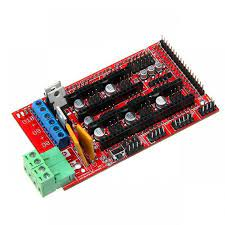
\includegraphics[scale=1]{4.jpg}}
    \caption{Плата RAMPS 1.4}
\end{figure}

В качестве шаговых двигателей используются двигатели 17HS4401S с драйверами Drv8825. Драйвер
Данный драйвер поддерживает ток до 2.2 А и 1/32 шага.

\begin{figure}[H]
    \center{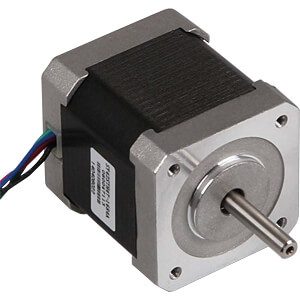
\includegraphics[scale=0.5]{5.jpg}}
    \caption{Двигатель 17HS4401S}
\end{figure}

\begin{figure}[H]
    \center{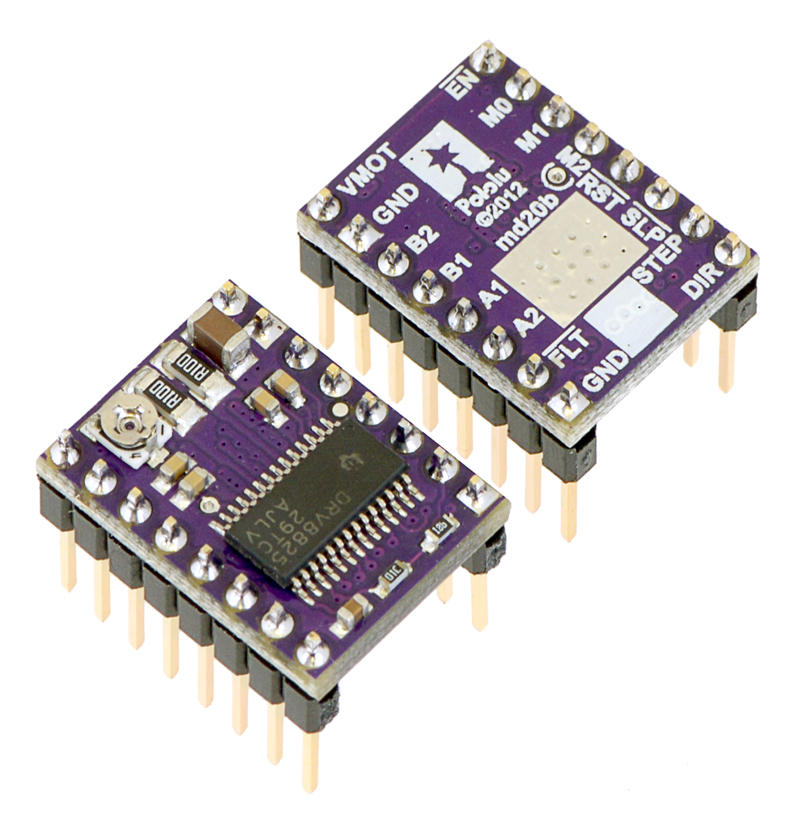
\includegraphics[scale=0.2]{6.jpg}}
    \caption{Драйвер Drv8825}
\end{figure}

Для более удобной работы с ЧПУ станком используется простой 4х
строчный LCD дисплей с SD card reader и с встроенным поворотным
энкодером RepRapDiscount Smart Controller.

\begin{figure}[H]
    \center{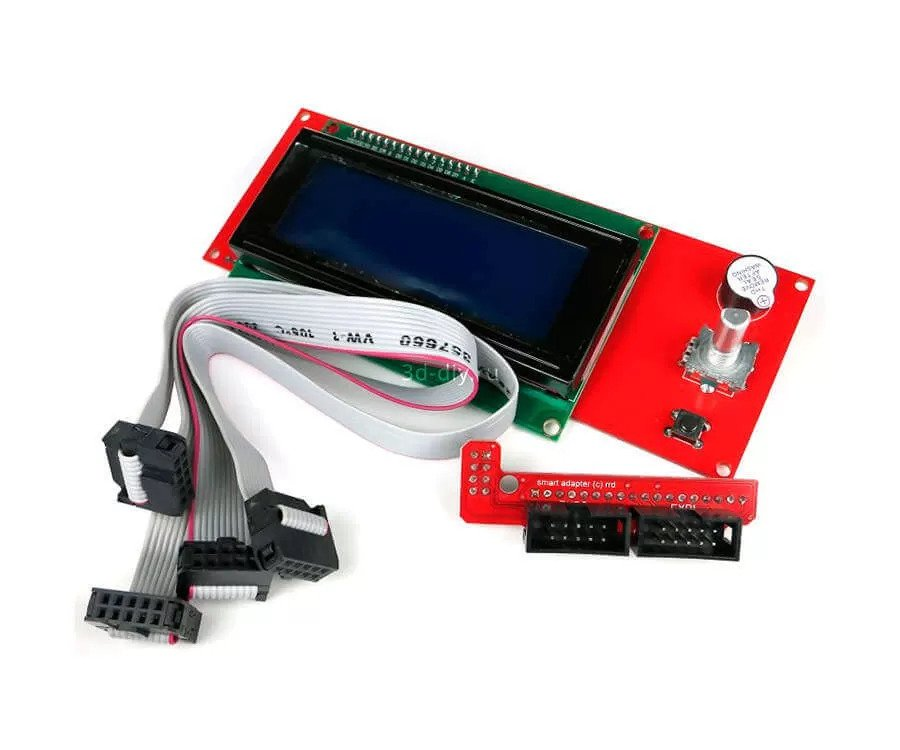
\includegraphics[scale=0.3]{7.jpg}}
    \caption{RepRapDiscount Smart Controller}
\end{figure}

% Все компоненты были собраны протестированы.

\begin{figure}[H]
    \center{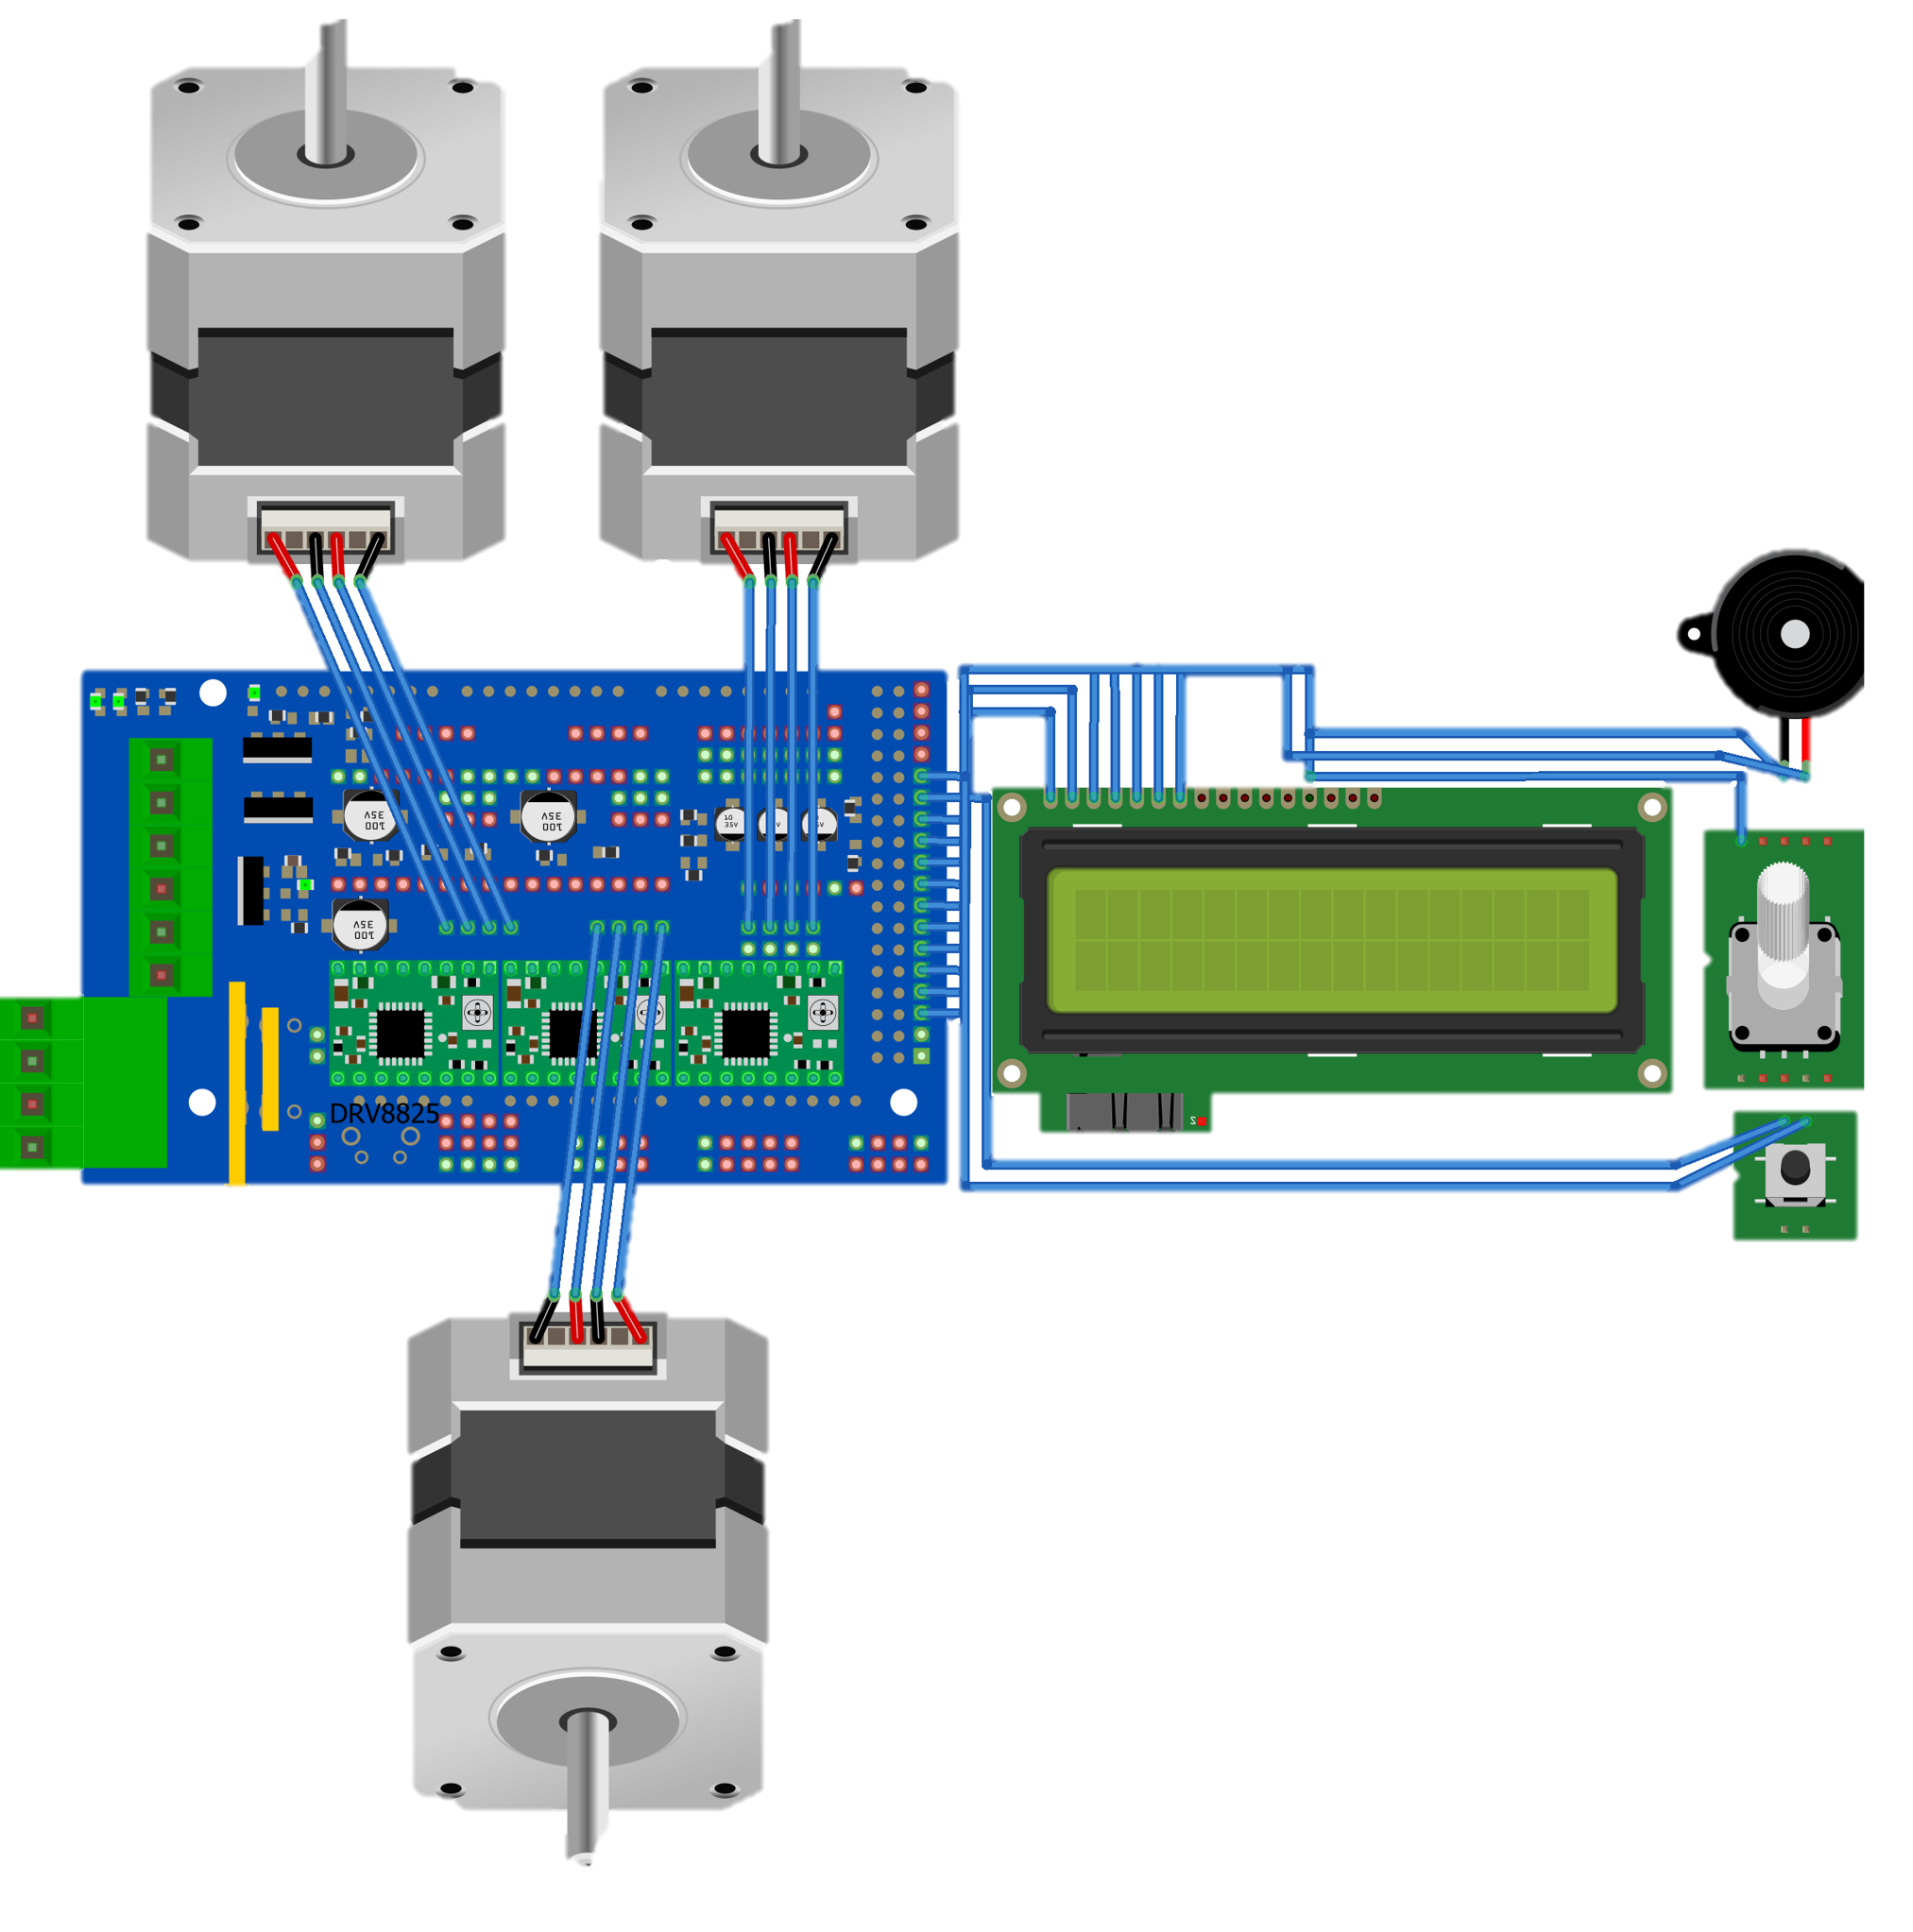
\includegraphics[scale=0.5]{8.png}}
    \caption{Схема компонентов}
\end{figure}

\section{Программная часть}

Поскольку основой нашего станка является железо от 3d принтера, в
качестве прошивки был выбран Marlin. Marlin - это прошивка с открытым
исходным кодом, гибрид от Sprinter и GRBL со множеством оригинальных
деталей и дополнений. Одним из ключей к популярности Marlin является то,
что он работает на 8-битных микроконтроллерах Atmel AVR. Эти чипы лежат
в основе популярной платформы Arduino с открытым исходным кодом.
Управляющий язык для Marlin является производным от G-code.
Поскольку прошивка специализируется для 3d принтеров требовалась настройки для работы в качестве ЧПУ станка.

Для получения G-code используется Fusion 360, однако для возможности работы с прошивкой Marlin требуется специальный постпроцессор \cite{themakermachine_mini}.
Загрузить его можно на странице \href{https://github.com/guffy1234/mpcnc_posts_processor}{github автора} и затем добавить в Fusion 360
в соответствии с официальной
\href{https://knowledge.autodesk.com/support/fusion-360/learn-explore/caas/sfdcarticles/sfdcarticles/How-to-add-a-Post-Processor-to-your-Personal-Posts-in-Fusion-360.html}{инструкцией}.
Важно при использовании данного программного инструмента с ЧПУ станком выставить правильные настройки для выхода оси z за пределы рабочей зоны.

\begin{figure}[H]
    \center{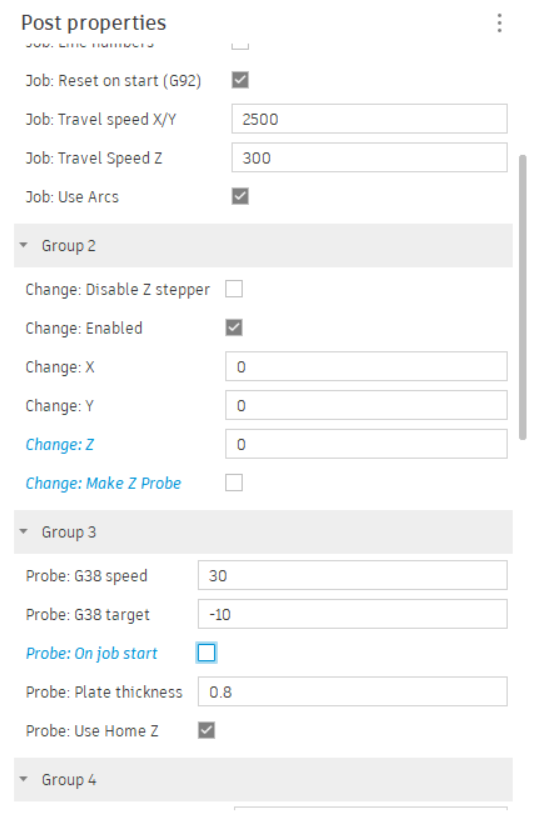
\includegraphics[scale=1]{9.png}}
    \caption{Настройки постпроцессора}
\end{figure}

\newpage
\bibliography{bibliography/bibliography}       %% имя библиографической базы (bib-файла) 

\end{document}